\tableofcontents

\newpage
\section{Performance evaluation of component-based software systems: A survey\cite{performance-model-survey}}

Durante los últimos diez años, los investigadores han propuesto muchos enfoques para evaluar el rendimiento (tiempos de respuesta, \emph{throughput}, utlización de recursos) de sistemas de software basados en componentes. Estos enfoques lidian con predicción de rendimiento y medición del rendimiento. Los primeros analizan el rendimiento esperado de un diseño de software basado en componentes para evitar problemas de rendimiento en la implementación del sistema, lo que podría llevar a costos substanciales para rediseñar la arquitectura. Los otros analizan el rendimiento observable de sistemas de software basados en componentes implementados para entender sus propiedades, determinar su capacidad máxima, identificar componentes críticos y para remover cuellos de botella.

\paragraph{\textbf{Métodos de evaluación de rendimiento}}
Los enfoques se agruparon en dos grandes grupos: enfoques principales que proporcionan procesos de evaluación de rendimiento completo y enfoques suplementarios que se centran en aspectos específicos como medición de componentes individuales o modelaje de las propiedades de rendimiento de los conectores de un componente.

\paragraph{Enfoques principales} 
\begin{itemize}
    \item Enfoques de predicción basados en UML:
    \begin{itemize}
        \item CB-SPE - \emph {The Component-Based Software Performance Engineering}
    \end{itemize}
    \item Enfoques de predicción basados en meta-modelos propietarios
    \begin{itemize}
        \item CBML - \emph{The Component-Based Modelling Language}
        \item PECT - \emph{The Prediction Enabled Component Technology}
        \item COMQUAD - \emph{Components with Quantitative properties and Adaptivity}
        \item KLAPPER
        \item ROBOCOP
        \item PALLADIO 
    \end{itemize}
    \item Enfoques de predicción centrados en \emph{middleware}
    \begin{itemize}
        \item NICTA
    \end{itemize}
    \item Enfoques basados en especificaciones formales
    \begin{itemize}
        \item RESOLVE
        \item HAMLET
    \end{itemize}
    \item Enfoques de monitoreo para sistemas implementados
    \begin{itemize}
        \item COMPAS
        \item TESTEJB
        \item AQUA
        \item PAD
    \end{itemize}
\end{itemize}

\paragraph{Enfoques Suplementarios}
\begin{itemize}
    \item Enfoques de monitoreo para componentes implementados
    \begin{itemize}
        \item RelCAM
        \item COMAERA
        \item BYCOUNTER
    \end{itemize}
    \item{Enfoques de predicción para conectores de componentes}
    \begin{itemize}
        \item Verdickt
        \item Grassi
        \item Becker
        \item Happe
    \end{itemize}
\end{itemize}
 


\newpage
\section{The Palladio component model for model-driven performance prediction\cite{palladio-seminal}}

El el desarrollo de software basado en componentes (CBSE, por sus siglas en inglés) la idea central es construir sistemas de software complejo uniendo componentes básicos. El objetivo inicial de CBSE fue incremetar el nivel de reutilización. Sin embargo, estructuras compuestas también pueden aumentar el nivel de predictibilidad del sistema durante etapas tempranas de desarrollo, esto porque modelos certificados de componentes individuales pueden ser compuestos, permitiendo a los arquitectos de software razonar sobre la estructura compuesta. Esto es importante para las propiedades funcionales, pero también para las propiedades extra funcionales como rendimiento y confiabilidad. 

Los métodos para predicción de rendimiento y confiabilidad de sistemas de software en general son limitados y raramente usados en la industria. Este reto es aún mayor en CBSE debido a que varios roles independientes están involucrados en la creación del sistema. Muchos métodos existentes para predicción de CBSE requieren que los arquitectos de software modelen el sistema basados en especificaciones de un solo componente. Luego se asume que el arquitecto proporcionará información faltante. Otros enfoques dejan de lado factores que afectan el rendimiento percibido de un componente de software tal y como la influencia de servicios externos, cambio de recursos de su ambiente o diferentes parámetros de entrada. Sin embargo, para predicciones precisas, todas estas dependencias tiene que hacerse explícitas en la especificación del componente.

Con \emph{Palladio\footnote{Toma su nombre del arquitecto renacentista Andrea Palladio (1508 - 1580) quien de cierta forma, intentó predecir el impacto estético de sus construcciones por adelantado.} Component Model} (PCM) un meta-modelo provee la especificación de información relevante del rendimiento de una arquitectura basada en componentes. El diseño y análisis de estos meta-modelos son los primeros que explícitamente incluyen todos los factores que influencian el rendimiento de un componente de software como lo son: la implementación, rendimiento de servicios externos, rendimiento del ambiente de ejecución y el perfil de uso. El modelo es diseñado con especial énfasis en la predicción de atributos de calidad de servicio como el rendimiento y la confiabilidad.

En el proceso de CBSE(figura \ref{fig:palladio-cbse}) los autores distinguen cuatro tipos de roles involucrados en la producción de artefactos de un sistema de software: \emph{desarrolladores de componentes} especifican e implementan los componentes, \emph{arquitectos de software} ensamblan componentes para construir aplicaciones, \emph{system deployers} modela los recursos del ambiente y luego su asignación, \emph{expertos del dominio de negocio} que están familiarizados con los usuarios del sistema y proporcionan modelos de su uso. El modelo completo del sistema puede ser derivado a partir de modelos parciales especificados por cada uno de los roles para que luego las propiedades extra funcionales puedan ser predecidas.

\begin{figure}[h!]
  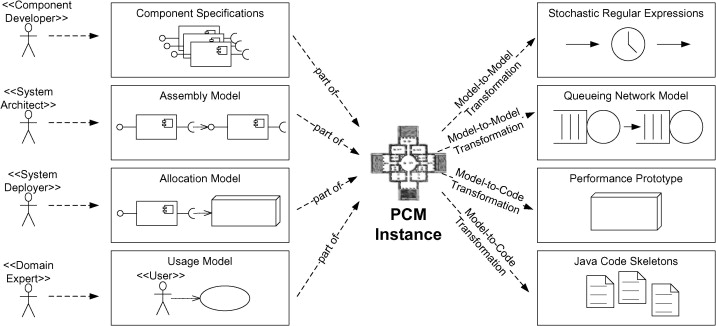
\includegraphics[width=8.7cm]{palladio-cbse-process}
  \caption{Proceso CBSE propuesto por PCM}
  \label{fig:palladio-cbse}
\end{figure} 


\newpage
\section{Performance-oriented DevOps: a research agenda\cite{performance-devops}}
DevOps es una tendencia hacia una estrecha integración entre equipos desarrollo y operaciones. La necesidad de tal integración es orientada por el requerimiento de adaptar aplicaciones empresariales a los cambios del ambiente del negocio continuamente. El rendimiento describe las propiedades del sistema con respecto a su ejecución y uso de recursos. Métricas comunes son tiempo de respuesta, \emph{throughput} y la utilización de los recursos. Los objetivos de rendimiento para aplicaciones empresariales son típicamente definidos al establecer cotas superiores/inferiores para estas métricas y transacciones de negocio específicas.

\subsection{Actividades de administración del rendimiento}
\subsubsection{Evaluación del rendimiento basado en modelos}
\begin{itemize}
    \item La representación de la memoria principal y del recolector de basura aún no están explícitamente integrados ni considerados en los modelos de rendimiento
    \item La selección de técnicas apropiadas de solución requiere de mucha experiencia
\end{itemize}

\subsubsection{Extracción de modelos de rendimiento y de cargas de trabajo}
\begin{itemize}
    \item La precisión de los modelos puede llegar a expirar si no son actualizados cuando hay cambios. Mecanismos de detección son requeridos para aprender cuando los modelos son antiguos y hay que actualizarlos.
    \item La extracción de capacidades de rendimiento se basa en una combinación de software y los recursos de hardware en los que se implementa. Este enfoque combinado es compatible con la precisión de la predicción, pero está menos calificado con respecto a la portabilidad de los conocimientos a otras plataformas. Una dirección de investigación futura podría ser extraer modelos separados (por ejemplo, \emph{middleware} y modelos de aplicación separados). 
\end{itemize}



\subsection{Ingeniería de rendimiento de software durante el desarrollo}

\subsubsection{Modelos de rendimiento durante etapas diseño }
\begin{itemize}
    \item Los retos de utilizar modelos de rendimiento en etapas tempranas de desarrollo es que usualmente es difícil validar la precisión de los modelos hasta que un sistema en ejecución exista. Las predicciones de rendimiento basadas en suposiciones, entrevistas y pruebas previas pueden ser también imprecisas y por tanto las decisiones que se hagan a partir de estas predicciones.
\end{itemize}


\paragraph{Sobre este reporte} Este es un reporte extenso que da a conocer retos y oportunidades en investigación sobre DevOps y rendimiento. En este resumen se incluyeron varios de los puntos más relevantes concernientes a modelaje del rendimiento. 





\newpage
\section{Performance Engineering for Microservices: Research Challenges and Directions\cite{microservices-challenges}}
Los microservicios complementan enfoques como DevOps y entrega continua(CD por sus siglas en inglés) en relación en términos de arquitectura de software. Junto con este estilo de arquitectura, otras tecnologías importantes para \emph{deployment} como, virtualización basada en contenedores y soluciones de orquestación de contenedores han emergido. Estas tecnologías permiten explotar plataformas en la nube, proporcionando altos niveles de escalabilidad, disponibilidad y portabilidad para microservicios. A pesar del hecho de que es una necesidad inherente contar con escalabilidad y elasticidad, la ingeniería de rendimiento para microservicios hasta ahora ha tenido poca atención por parte de las comunidades tanto de microservicios como de comunidades de investigación de ingeniería de rendimiento. Un gran cuepro de conocimiento y buenas prácticas para ingeniería de rendimiento para desarrollo tradicional de software y arquitecturas está disponible. Sin embargo, sus aplicaciones en DevOps imponen tanto retos como oportunidades.

\subsection{Retos de investigación}

\subsubsection{Pruebas de rendimiento}
\begin{itemize}
    \item Reemplazar y compensar pruebas extensivas de integración y de sistema por un control detallado de los entornos de producción
    \item Alinear las pruebas de rendimiento y pruebas de regresión de rendimiento con prácticas de entrega continua, por ejemplo, acelerar las estas de pruebas correspondientes.
    \item Selección dinámica y semi automática de pruebas de rendimiento
\end{itemize}

\subsubsection{Monitoreo}
\begin{itemize}
    \item Instrumentación para monitoreo distribuido arquitecturas microservicios políglotas 
    \item Métricas adicionales para monitorear microservicios
    \item Técnicas de detección precisa de anomalías en arquitecturas de microservicios
\end{itemize}


\subsubsection{Modelado del rendimiento}
De momento no existen enfoques para modelado del rendimiento de microservicios 
\begin{itemize}
    \item Adoptar modelos de rendimiento para casos de uso como planeamiento de capacidad, confiabilidad y resiliencia
    \item Buscar abstracciones de modelado apropiadas 
    \item Extracción automática de modelos de rendimiento
    \item Aprender del comportamiento de la infraestructura e integrarlo en los modelos de rendimiento
\end{itemize}






\newpage
\section{An industrial case study of performance and cost design space exploration\cite{case-study-1}}

Determinar la compensación(\emph{trade-off}) entre rendimiento y costo de un sistema de software distribuido es importante ya que permite cumplir los requerimientos de rendimiento de una forma rentable. La gran cantidad de alternativas de diseño para tales sistemas usualmente llevan a los arquitectos de software a seleccionar soluciones subóptimas, las cuales puede desperdiciar recursos o no hacerle frente a las cargas de trabajo futuras. 

La mayor contribución de este artículo es un caso de estudio que presenta la aplicación de varias herramientas y métodos académicos para la exploración de diseños en un ambiente industrial. El caso de estudio presenta cómo se exploran lo cambios en replicación, reasignación(\emph{reallocation} y hardware y su implicación en costo y rendimiento. 
\paragraph{Sistema en estudio} Una solución de diagnóstico remoto (RDS por sus siglas en inglés) de la compañía ABB. El sistema RDS tiene más de 150000 líneas de código y es usado para actividades de servicio en miles de dispositivos industriales, fallas y otros datos. ABB desea mejorar el rendimiento de RDS con una nueva arquitectura porque su \emph{back-end} está operando en sus límites de rendimiento y escalabilidad. Las mejoras de corto plazo en el rendimiento y hardware no resolverán de forma sostenible los problemas a largo plazo. La métrica de mayor interés para los \emph{stakeholders} del sistema es el rendimiento de carga(\emph{upload}) del dispositivo, por ejemplo, el número de cargas que el sistema pueda manejar por segundo. Se decidió que el sistema en promedio no debe utilizar más del 50\% de recursos para hacerle frente a las cargas de trabajo pico.

\paragraph{Actividades} 3 principales actividades se llevaron a cabo: medición del rendimiento, modelado del rendimiento y exploración de diseños candidatos.

\subsection{Medición del rendimiento}
Mediciones son necesarias para crear un modelo de rendimiento preciso. Para medir el rendimiento de RDS de forma precisa, varios paso fueron realizados: primero se seleccionaron las herramientas para la medición, luego se creó un modelo de la carga de trabajo del sistema. Finalmente, se realizaron las mediciones.

\subsection{Modelado del rendimiento}
Para construir el modelo del rendimiento de RDS, primero se seleccionó una notación de modelaje apropiada que resultó ser el \emph{Palladio Component Model}. Basado en los resultados de las mediciones, el modelo de la carga de trabajo y análisis adicionales, se construyó un modelo de Palladio para el RDS, el cual se calibró hasta que reflejará el rendimiento del sistema en estudio.

\subsection{Exploración de diseños candidatos}
Basado en la modelo del rendimiento creado, se buscó la arquitectura más eficiente en costo para hacerle frente a la carga de trabajo incremental. Se consideraron 3 escenarios y para cada uno de ellos se determinó la arquitectura adecuada que cumpliera con el objetivo de rendimiento. Se ejecutaron varias predicciones manuales para calibrar el modelo. Debido a la gran cantidad de soluciones, se aplicó un herramienta de exploración de diseños candidatos llamada \emph{PerOpteryx}. Se ejecutaron varias predicciones y se creó un plan para aplicar las arquitecturas.


\newpage
\section{Sobre la propuesta}
Los artículos incluidos se podrían llegar a dividir en dos grupos: los que destacan la investigación reciente y generalidades sobre modelaje de rendimiento en sistemas de software, haciendo énfasis en \emph{Palladio Component Model}, y los que dan a conocer retos y oportunidades alrededor de estos temas con respecto a tendencias de desarrollo de software actuales como lo es DevOps.

Se incluye también un caso de estudio en el cual a través del uso de herramientas de modelaje de rendimiento, un sistema es analizado y de acuerdo con los resultados obtenidos se proponen arquitecturas optimizadas. Otros ejemplos de casos de uso relacionados con modelaje y predicciones del rendimiento se pueden encontrar en \cite{huber-et-al, rathfelder-et-al, media-store}.

A partir de lo recolectado se pudo conocer que mucho del esfuerzo que se ha hecho en este campo de estudio ha tenido baja aceptación en la industria pero que, por otro lado, compañías y sistemas que han utilizado estos métodos de modelaje y evaluación han obtenido buenos resultados. Queda claro también que la aplicación de estos modelos permiten entender la influencia que tienen tanto de los diferentes componentes de software como el impacto que pudiera generar en ellos durante la ejecución de un sistema.

También se pudo reconocer que existe necesidad en aplicar enfoques de modelado del rendimiento en el desarrollo de sistemas modernos. No existen enfoques de modelado de rendimiento para microservicios que hoy en día es un estilo de arquitectura de software sumamente popular. Es por esto que se considera que la realización de estudios exploratorios para determinar la influencia en el rendimiento que tienen diferentes componentes, librerías y productos de software sobre un sistema van a brindar nuevo conocimiento para dar a conocer factores que favoren o desfavorecen el uso de los mismos y, además de esto, podría representar un marco de referencia inicial por medio del cual se pueda evaluar la adopción de estas tecnologías \emph{a priori}. 

Por último, durante la búsqueda de artículos se encontraron muy pocos de ellos provenientes de universidades de latinoamérica. Esto representa, a juicio del proponente, una oportunidad para estudiar, probar y generar conocimiento sobre estos temas.    


\section{Objetivos}

\subsection{Objetivo General}
Diseñar un modelo de sistemas distribuidos de intercambio mensajes (\emph{message-oriented middleware}) para evaluar la influencia que tienen en el rendimiento de un sistema de software por medio de modelado y simulación basado en componentes.

\subsection{Objetivos Específicos}
\begin{enumerate}
    \item Adaptar un sistema de software de referencia para el cual ya exista un modelo de rendimiento y simulaciones para que se integre y comunique con un sistema de mensajería.
    \item Comparar la solución implementada bajo diferentes cargas de trabajo
    \item Crear un modelo del nuevo sistema y su rendimiento 
    \item Validar y analizar el modelo creado a través de experimentos
\end{enumerate}



\newpage
\bibliographystyle{ACM-Reference-Format}
\begin{thebibliography}{9}

\bibitem{performance-model-survey} Heiko Koziolek. 2010. \emph{Performance evaluation of component-based software systems: A survey. Perform}. Eval. 67, 8 (August 2010), 634-658. DOI: \url{http://ezproxy.itcr.ac.cr:2075/10.1016/j.peva.2009.07.007} 

\bibitem{palladio-seminal} Stephen Becker, Heiko Koziolek and Ralf Reussner. \emph{The Palladio component model for model-driven prediction}. Journal of Systems and Software 82:3-22. Elsevier Science Inc. 2009. DOI: \url{http://dx.doi.org/10.1016/j.jss.2008.03.066}

\bibitem{performance-devops} Andreas Brunnert, André van Hoorn, Felix Willnecker, Alexandru Danciu, Wilhelm Hasselbring, Christoph Heger, Nikolas Roman Herbst, Pooyan Jamshidi, Reiner Jung, Jóakim von Kistowski, Anne Koziolek, Johannes Kroß, Simon Spinner, Christian Vögele, Jürgen Walter, and Alexander Wert. \emph{Performance-oriented devops: A research agenda}. Technical Report SPEC-RG-2015-01, SPEC Research Group - DevOps Performance Working Group, Standard Performance Evaluation Corporation (SPEC), 2015. \url{http://arxiv.org/abs/1508.04752}

\bibitem{microservices-challenges} Robert Heinrich, André van Hoorn, Holger Knoche, Fei Li, Lucy Ellen Lwakatare, Claus Pahl, Stefan Schulte, and Johannes Wettinger. \emph{Performance engineering for microservices: Research challenges and directions}. In Companion Proceedings of the 8th ACM/SPEC on International Conference on Performance Engineering, 2017, pages 223-226. DOI: \url{https://doi.org/10.1145/3053600.3053653}

\bibitem{case-study-1} Thijmen de Gooijer, Anton Jansen, Heiko Koziolek, and Anne Koziolek. 2012. \emph{An industrial case study of performance and cost design space exploration}. In Proceedings of the 3rd ACM/SPEC International Conference on Performance Engineering (ICPE '12). ACM, New York, NY, USA, 205-216. DOI: \url{https://ezproxy.itcr.ac.cr:2878/10.1145/2188286.2188319}

\bibitem{huber-et-al} Nikolaus Huber, Steffen Becker, Christoph Rathfelder, Jochen Schweflinghaus, and Ralf H. Reussner. 2010. \emph{Performance modeling in industry: a case study on storage virtualization}. In Proceedings of the 32nd ACM/IEEE International Conference on Software Engineering - Volume 2 (ICSE '10), Vol. 2. ACM, New York, NY, USA, 1-10. DOI: \url{http://ezproxy.itcr.ac.cr:2075/10.1145/1810295.1810297} 

\bibitem{rathfelder-et-al} Christoph Rathfelder, Steffen Becker, Klaus Krogmann and Ralf Reussner. \emph{Workload-aware System Monitoring Using Performance Predictions Applied to a Large-scale E-Mail System}. 2012 Joint Working IEEE/IFIP Conference on Software Architecture and European Conference on Software Architecture, Helsinki, 2012, pp. 31-40.
DOI: \href{https://ezproxy.itcr.ac.cr:2878/10.1109/WICSA-ECSA.212.11}{10.1109/WICSA-ECSA.212.11}. 

\bibitem{media-store} Misha Strittmatter and Amine Kechaou. \emph{The media store 3 case study system}. Technical Report 2016,1, Faculty of Informatics, Karlsruhe Institute of Technology, 2016. URL: \url{http://digbib.ubka.uni-karlsruhe.de/volltexte/documents/3792054}

\end{thebibliography}

%\appendix
%\section{}


%\section{Introduction}
%
%
%As a new technology, Wireless Sensor Networks (WSNs) has a wide
%range of applications \cite{Culler-01, Bahl-02, Akyildiz-01}, including
%environment monitoring, smart buildings, medical care, industrial and
%military applications. Among them, a recent trend is to develop
%commercial sensor networks that require pervasive sensing of both
%environment and human beings, for example, assisted living
%\cite{Akyildiz-02, Harvard-01,CROSSBOW} and smart homes
%\cite{Harvard-01, Adya-01,CROSSBOW}.
% quote
%\begin{quote}
%  ``For these applications, sensor devices are incorporated into human
%  cloths \cite{Natarajan-01, Zhou-06, Bahl-02, Adya-01} for monitoring
%  health related information like EKG readings, fall detection, and
%  voice recognition''.
%\end{quote}
%While collecting all these multimedia information
%\cite{Akyildiz-02} requires a high network throughput, off-the-shelf
%sensor devices only provide very limited bandwidth in a single
%channel: 19.2\,Kbps in MICA2 \cite{Bahl-02} and 250\,Kbps in MICAz.
%
%In this article, we propose MMSN, abbreviation for Multifrequency
%Media access control for wireless Sensor Networks. The main
%contributions of this work can be summarized as follows.
% itemize
%\begin{itemize}
%\item To the best of our knowledge, the MMSN protocol is the first
%multifrequency MAC protocol especially designed for WSNs, in which
%each device is equipped with a single radio transceiver and
%the MAC layer packet size is very small.
%\item Instead of using pairwise RTS/CTS frequency negotiation
%\cite{Adya-01, Culler-01, Tzamaloukas-01, Zhou-06},
%we propose lightweight frequency assignments, which are good choices
%for many deployed comparatively static WSNs.
%\item We develop new toggle transmission and snooping techniques to
%enable a single radio transceiver in a sensor device to achieve
%scalable performance, avoiding the nonscalable ``one
%control channel + multiple data channels'' design \cite{Natarajan-01}.
%\end{itemize}
%
% Head 1
%\section{MMSN Protocol}
%
% Head 2
%\subsection{Frequency Assignment}
%
%We propose a suboptimal distribution to be used by each node, which is
%easy to compute and does not depend on the number of competing
%nodes. A natural candidate is an increasing geometric sequence, in
%which
% Numbered Equation
%\begin{equation}
%\label{eqn:01}
%P(t)=\frac{b^{\frac{t+1}{T+1}}-b^{\frac{t}{T+1}}}{b-1},
%\end{equation}
%where $t=0,{\ldots}\,,T$, and $b$ is a number greater than $1$.
%
%In our algorithm, we use the suboptimal approach for simplicity and
%generality. We need to make the distribution of the selected back-off
%time slice at each node conform to what is shown in
%Equation~\eqref{eqn:01}. It is implemented as follows: First, a random
%variable $\alpha$ with a uniform distribution within the interval $(0,
%1)$ is generated on each node, then time slice $i$ is selected
%according to the following equation:
% Unnumbered Equation
%\[
%i=\lfloor(T+1)\log_b[\alpha(b-1)+1]\rfloor.
%\]
%It can be easily proven that the distribution of $i$ conforms to Equation
%(\ref{eqn:01}).
%
%So protocols \cite{Bahl-02, Culler-01,Zhou-06,Adya-01,
%Tzamaloukas-01, Akyildiz-01} that use RTS/CTS
%controls\footnote{RTS/CTS controls are required to be implemented by
%802.11-compliant devices. They can be used as an optional mechanism
%to avoid Hidden Terminal Problems in the 802.11 standard and
%protocols based on those similar to \cite{Akyildiz-01} and
%\cite{Adya-01}.} for frequency negotiation and reservation are not
%suitable for WSN applications, even though they exhibit good
%performance in general wireless ad-hoc
%networks.
%
% Head 3
%\subsubsection{Exclusive Frequency Assignment}
%
%
%In exclusive frequency assignment, nodes first exchange their IDs
%among two communication hops so that each node knows its two-hop
%neighbors' IDs. In the second broadcast, each node beacons all
%neighbors' IDs it has collected during the first broadcast period.
%
% Head 4
%\paragraph{Eavesdropping}
%
%Even though the even selection scheme leads to even sharing of
%available frequencies among any two-hop neighborhood, it involves a
%number of two-hop broadcasts. To reduce the communication cost, we
%propose a lightweight eavesdropping scheme.
%
%\subsection{Basic Notations}
%
%As Algorithm~\ref{alg:one} states, for each frequency
%number, each node calculates a random number (${\textit{Rnd}}_{\alpha}$) for
%itself and a random number (${\textit{Rnd}}_{\beta}$) for each of its two-hop
%neighbors with the same pseudorandom number generator.
%
% Algorithm
%\begin{algorithm}[t]
%\SetAlgoNoLine
%\KwIn{Node $\alpha$'s ID ($ID_{\alpha}$), and node $\alpha$'s
%neighbors' IDs within two communication hops.}
%\KwOut{The frequency number ($FreNum_{\alpha}$) node $\alpha$ gets assigned.}
%$index$ = 0; $FreNum_{\alpha}$ = -1\;
%\Repeat{$FreNum_{\alpha} > -1$}{
%        $Rnd_{\alpha}$ = Random($ID_{\alpha}$, $index$)\;
%        $Found$ = $TRUE$\;
%        \For{each node $\beta$ in $\alpha$'s two communication hops
%    }{
%      $Rnd_{\beta}$ = Random($ID_{\beta}$, $index$)\;
%      \If{($Rnd_{\alpha} < Rnd_{\beta}$) \text{or} ($Rnd_{\alpha}$ ==
%          $Rnd_{\beta}$ \text{and} $ID_{\alpha} < ID_{\beta}$)\;
%      }{
%        $Found$ = $FALSE$; break\;
%      }
%        }
%     \eIf{$Found$}{
%           $FreNum_{\alpha}$ = $index$\;
%         }{
%           $index$ ++\;
%     }
%      }
%\caption{Frequency Number Computation}
%\label{alg:one}
%\end{algorithm}
%
%
%Bus masters are divided into two disjoint sets, $\mathcal{M}_{RT}$
%and $\mathcal{M}_{NRT}$.
% description
%\begin{description}
%\item[RT Masters]
%$\mathcal{M}_{RT}=\{ \vec{m}_{1},\dots,\vec{m}_{n}\}$ denotes the
%$n$ RT masters issuing real-time constrained requests. To model the
%current request issued by an $\vec{m}_{i}$ in $\mathcal{M}_{RT}$,
%three parameters---the recurrence time $(r_i)$, the service cycle
%$(c_i)$, and the relative deadline $(d_i)$---are used, with their
%relationships.
%\item[NRT Masters]
%$\mathcal{M}_{NRT}=\{ \vec{m}_{n+1},\dots,\vec{m}_{n+m}\}$ is a set
%of $m$ masters issuing nonreal-time constrained requests. In our
%model, each $\vec{m}_{j}$ in $\mathcal{M}_{NRT}$ needs only one
%parameter, the service cycle, to model the current request it
%issues.
%\end{description}
%
%Here, a question may arise, since each node has a global ID. Why
%don't we just map nodes' IDs within two hops into a group of
%frequency numbers and assign those numbers to all nodes within two
%hops?
%
%\section{Simulator}
%\label{sec:sim}
%
%If the model checker requests successors of a state which are not
%created yet, the state space uses the simulator to create the
%successors on-the-fly. To create successor states the simulator
%conducts the following steps.
% enumerate
%\begin{enumerate}
%\item Load state into microcontroller model.
%\item Determine assignments needed for resolving nondeterminism.
%\item For each assignment.
%      \begin{enumerate}
%      \item either call interrupt handler or simulate effect of next instruction, or
%      \item evaluate truth values of atomic propositions.
%      \end{enumerate}
%\item Return resulting states.
%\end{enumerate}
%Figure~\ref{fig:one} shows a typical microcontroller C program that
%controls an automotive power window lift. The program is one of the
%programs used in the case study described in Section~\ref{sec:sim}.
%At first sight, the programs looks like an ANSI~C program. It
%contains function calls, assignments, if clauses, and while loops.
% Figure
%\begin{figure}
%  
\includegraphics{mouse}
%  \caption{Code before preprocessing.}
%  \label{fig:one}
%\end{figure}
%
%\subsection{Problem Formulation}
%
%The objective of variable coalescence-based offset assignment is to find
%both the coalescence scheme and the MWPC on the coalesced graph. We start
%with a few definitions and lemmas for variable coalescence.
%
% Enunciations
%\begin{definition}[Coalesced Node (C-Node)]A C-node is a set of
%live ranges (webs) in the AG or IG that are coalesced. Nodes within the same
%C-node cannot interfere with each other on the IG. Before any coalescing is
%done, each live range is a C-node by itself.
%\end{definition}
%
%\begin{definition}[C-AG (Coalesced Access Graph)]The C-AG is the access
%graph after node coalescence, which is composed of all C-nodes and C-edges.
%\end{definition}
%
%\begin{lemma}
%The C-MWPC problem is NP-complete.
%\end{lemma}
%\begin{proof} C-MWPC can be easily reduced to the MWPC problem assuming a
%coalescence graph without any edge or a fully connected interference graph.
%Therefore, each C-node is an uncoalesced live range after value separation
%and C-PC is equivalent to PC. A fully connected interference graph is made
%possible when all live ranges interfere with each other. Thus, the C-MWPC
%problem is NP-complete.
%\end{proof}
%
%\begin{lemma}[Lemma Subhead]The solution to the C-MWPC problem is no
%worse than the solution to the MWPC.
%\end{lemma}
%\begin{proof}
%Simply, any solution to the MWPC is also a solution to the
%C-MWPC. But some solutions to C-MWPC may not apply to the MWPC (if any
%coalescing were made).
%\end{proof}
%
%\section{Performance Evaluation}
%
%During all the experiments, the Geographic Forwarding (GF) by Akyildiz
%et al.~\shortcite{Akyildiz-01} routing protocol is used. GF exploits
%geographic information of nodes and conducts local data-forwarding to
%achieve end-to-end routing. Our simulation is configured according to
%the settings in Table~\ref{tab:one}. Each run lasts for 2 minutes and
%repeated 100 times. For each data value we present in the results, we
%also give its 90\% confidence interval.
%
% Table
%\begin{table}%
%\caption{Simulation Configuration}
%\label{tab:one}
%\begin{minipage}{\columnwidth}
%\begin{center}
%\begin{tabular}{ll}
%  \toprule
%  TERRAIN\footnote{This is a table footnote. This is a
%    table footnote. This is a table footnote.}   & (200m$\times$200m) Square\\
%  Node Number     & 289\\
%  Node Placement  & Uniform\\
%  Application     & Many-to-Many/Gossip CBR Streams\\
%  Payload Size    & 32 bytes\\
%  Routing Layer   & GF\\
%  MAC Layer       & CSMA/MMSN\\
%  Radio Layer     & RADIO-ACCNOISE\\
%  Radio Bandwidth & 250Kbps\\
%  Radio Range     & 20m--45m\\
%  \bottomrule
%\end{tabular}
%\end{center}
%\bigskip\centering
%\footnotesize\emph{Source:} This is a table
% sourcenote. This is a table sourcenote. This is a table
% sourcenote.
%
% \emph{Note:} This is a table footnote.
%\end{minipage}
%\end{table}%
%
%
%\section{Conclusions}
%
%In this article, we develop the first multifrequency MAC protocol for
%WSN applications in which each device adopts a
%single radio transceiver. The different MAC design requirements for
%WSNs and general wireless ad-hoc networks are
%compared, and a complete WSN multifrequency MAC design (MMSN) is
%put forth. During the MMSN design, we analyze and evaluate different
%choices for frequency assignments and also discuss the nonuniform
%back-off algorithms for the slotted media access design.
%
% Start of "Sample References" section
%
%\section{Typical References in New ACM Reference Format}
%A paginated journal article \cite{Abril07}, an enumerated
%journal article \cite{Cohen07}, a reference to an entire issue \cite{JCohen96},
%a monograph (whole book) \cite{Kosiur01}, a monograph/whole book in a series (see 2a in spec. document)
%\cite{Harel79}, a divisible-book such as an anthology or compilation \cite{Editor00}
%followed by the same example, however we only output the series if the volume number is given
%\cite{Editor00a} (so Editor00a's series should NOT be present since it has no vol. no.),
%a chapter in a divisible book \cite{Spector90}, a chapter in a divisible book
%in a series \cite{Douglass98}, a multi-volume work as book \cite{Knuth97},
%an article in a proceedings (of a conference, symposium, workshop for example)
%(paginated proceedings article) \cite{Andler79}, a proceedings article
%with all possible elements \cite{Smith10}, an example of an enumerated
%proceedings article \cite{VanGundy07},
%an informally published work \cite{Harel78}, a doctoral dissertation \cite{Clarkson85},
%a master's thesis: \cite{anisi03}, an online document / world wide web
%resource \cite{Thornburg01, Ablamowicz07, Poker06}, a video game (Case 1) \cite{Obama08} and (Case 2) \cite{Novak03}
%and \cite{Lee05} and (Case 3) a patent \cite{JoeScientist001},
%work accepted for publication \cite{rous08}, 'YYYYb'-test for prolific author
%\cite{SaeediMEJ10} and \cite{SaeediJETC10}. Other cites might contain
%'duplicate' DOI and URLs (some SIAM articles) \cite{Kirschmer:2010:AEI:1958016.1958018}.
%Boris / Barbara Beeton: multi-volume works as books
%\cite{MR781536} and \cite{MR781537}.
%
%A couple of citations with DOIs: \cite{2004:ITE:1009386.1010128,
%  Kirschmer:2010:AEI:1958016.1958018}.
%
%Online citations: \cite{TUGInstmem, Thornburg01, CTANacmart}.
%
% Appendix
%\appendix
%\section{Switching Times}
%
%In this appendix, we measure the channel switching time of Micaz
%\cite{CROSSBOW} sensor devices.  In our experiments, one mote
%alternatingly switches between Channels~11 and~12. Every time after
%the node switches to a channel, it sends out a packet immediately and
%then changes to a new channel as soon as the transmission is finished.
%We measure the number of packets the test mote can send in 10 seconds,
%denoted as $N_{1}$. In contrast, we also measure the same value of the
%test mote without switching channels, denoted as $N_{2}$. We calculate
%the channel-switching time $s$ as
%\begin{displaymath}%
%s=\frac{10}{N_{1}}-\frac{10}{N_{2}}.
%\end{displaymath}%
%By repeating the experiments 100 times, we get the average
%channel-switching time of Micaz motes: 24.3\,$\mu$s.
%
%\section{Supplementary Materials}
%
%
%\begin{printonly}
%  See the supplementary materials in the online version
%\end{printonly}
%
%\begin{screenonly}
%\subsection{This is an Example of Appendix Subsection Head}
%
%Channel-switching time is measured as the time length it takes for
%motes to successfully switch from one channel to another. This
%parameter impacts the maximum network throughput, because motes
%cannot receive or send any packet during this period of time, and it
%also affects the efficiency of toggle snooping in MMSN, where motes
%need to sense through channels rapidly.
%
%By repeating experiments 100 times, we get the average
%channel-switching time of Micaz motes: 24.3 $\mu$s. We then conduct
%the same experiments with different Micaz motes, as well as
%experiments with the transmitter switching from Channel 11 to other
%channels. In both scenarios, the channel-switching time does not have
%obvious changes. (In our experiments, all values are in the range of
%23.6 $\mu$s to 24.9 $\mu$s.)
%
%\subsection{Appendix Subsection Head}
%
%The primary consumer of energy in WSNs is idle listening. The key to
%reduce idle listening is executing low duty-cycle on nodes. Two
%primary approaches are considered in controlling duty-cycles in the
%MAC layer.
%
%\end{screenonly}
%
%\begin{acks}
%
%The authors would like to thank Dr. Maura Turolla of Telecom
%Italia for providing specifications about the application scenario.
%
%The work is supported by the \grantsponsor{GS501100001809}{National
%  Natural Science Foundation of
%  China}{http://dx.doi.org/10.13039/501100001809} under Grant
%No.:~\grantnum{GS501100001809}{61273304\_a}
%and~\grantnum[http://www.nnsf.cn/youngscientists]{GS501100001809}{Young
%  Scientists' Support Program}.
%
%
%\end{acks}
%
% Bibliography
%\bibliographystyle{ACM-Reference-Format}
%\bibliography{sample-bibliography}
